\chapter[Appendix]{Appendix: summaries of additional papers not presented
  in this thesis}

The following is a chronological list of papers
that include direct contributions from myself and have not been included as
chapters in this thesis. Lead author papers in the following subsections 
are accompanied by a brief paper
summary whereas papers for which I was a contributing author are accompanied by
descriptions of those contributions.

\section{Prospects for Detecting the Rossiter-McLaughlin Effect of
  Earth-like Planets: the test case of TRAPPIST-1b and c \citep{cloutier16a}}
The Rossiter-McLaughlin (RM) effect, or spectroscopic transit, is an observable
effect that is sensitive to the sky-projected spin-orbit angle $\lambda$ of a
planet's orbital plane relative to the host star's spin axis (see
Fig.~\ref{fig:RMillust}). The measurement of $\lambda$ may
be used to inform formation models and planet dynamical histories. Notably, it
has yet to be measured for any terrestrial-sized exoplanet ($\lesssim 1.6$ R$_{\oplus}$)
owing to their typically shallow transit depths. 
In this paper, which followed shortly after the discovery of at least three
terrestrial-sized planets orbiting the ultracool dwarf TRAPPIST-1 
\citep{gillon16}, we
argued that the two innermost planets represent ideal targets for being
the best terrestrial-sized exoplanets amenable to the detection of the RM effect
discovered to date.
Due to the small size of TRAPPIST-1, its short rotation period (i.e. large \vsini{)}, and its
relatively low level of activity compared to other ultracool dwarfs, we expect
the semi-amplitudes of the TRAPPIST-1b and c RM effects to be $\sim 40-50$
\mps{} which is an order of magnitude greater than the amplitude of the
Doppler reflex motion induced by the planets on their host star.
Simulations of the RM effect showed that if the planets are
well-aligned, then $\lambda$ can be measured with a precision of
$\lesssim 10^{\circ}$ in an RV time series with typical measurement
uncertainties of 2 \mps{,} although multiple transits will be required due to the faintness
of TRAPPIST-1 ($J=11.4$).

\begin{figure}
  \centering
  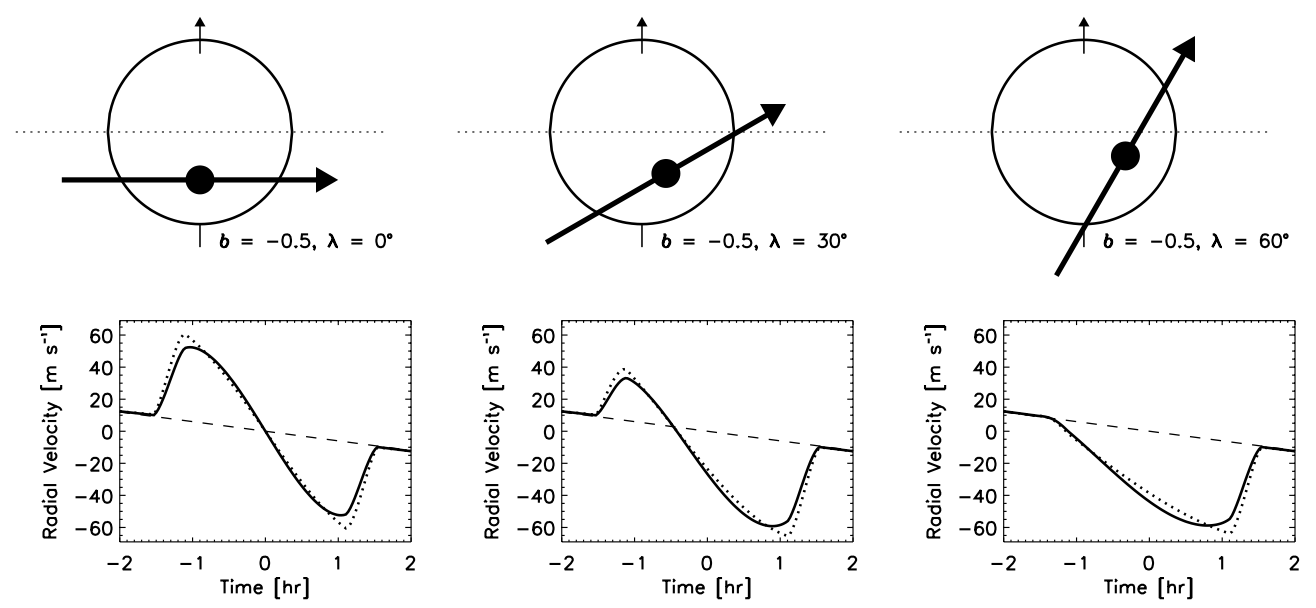
\includegraphics[width=.9\textwidth]{figures/RMeffect.png}
  \caption[Measuring the sky-projected spin-orbit angle using the RM effect.]
          {Dependence of the anomalous RV waveform from the
            Rossiter-McLaughlin effect on the sky-projected spin-orbit angle
            $\lambda$. All depicted trajectories during the planetary transit
            have the same impact parameter $b=-0.5$. The solid and dashed curves
            correspond to different assumed limb darkening coefficients. 
          \citep[Image credit:][]{gaudi07}}
  \label{fig:RMillust}
\end{figure}


\section{On the Radial Velocity Detection of Additional Planets in Transiting,
  Slowly Rotating M dwarf Systems: The Case of GJ 1132 \citep{cloutier17a}}
\label{app:gj1132}
M dwarfs are known to frequently host multi-planet systems such that we can
reasonably expect to find additional planets with RVs around M dwarfs that
are known to host at
least one transiting planet. In this paper we focused on one such
system, namely the nearby mid-M dwarf GJ 1132, which hosts a small transiting
planet at $P=1.6$ days. This system is amenable to deep RV follow-up both for
the precise mass measurement of GJ 1132b and for the search for non-transiting
planets in the system. We created synthetic RV time series
by injecting planets from the empirical M dwarf occurrence rates plus physical
models of stellar activity. We then applied our GP formalism for modelling
stellar activity (Sect.~\ref{sect:gp}) to attempt to recover those planets.
From these calculations we compute our sensitivity to the detection of additional
planets in the GJ 1132 planetary system as a function of the number of RV
measurements. We show that at 1 \mps{} precision, $\sim 50$\% of all non-transiting
planets from the expected planet population can be detected with $\sim 50$
measurements. \\

Indeed there turns out to be at least one additional planet in the GJ 1132
planetary system
that is not transiting and is presented in Sect.~\ref{sect:gj1132bonfils}.

\section{Near-InfraRed Planet Searcher to Join HARPS on the ESO 3.6-metre
  Telescope \citep{bouchy17}}
This paper summarized the current status of the up-coming near-IR spectrograph
NIRPS (\emph{Near-InfraRed Planet Searcher}) including an overview of its design
and primary science goals. As an instrument paper all science team members were
added as co-authors including myself as a Canadian collaborator. I did however
contribute directly to the discussion of the NIRPS science goal of searching
for new RV planetary systems in the southern sky that may be amenable to direct
imaging with ELTs. Those specific contributions were calculations of the
expected NIRPS planet yield. These calculations were based on the simulations
presented in Chapter~\ref{chap:BS} for the
SPIRou Legacy Survey-Planet Search after modifications to the simulated
observing strategy and instrument performance were made as they pertain to
NIRPS.


\section{Quantifying the Evidence for a Planet in Radial Velocity Data
  \citep{nelson18}}
The paper presents the results of a collaborative study that was conceived in
a breakout session during the \emph{Extremely Precise Radial Velocities III}
conference at Penn State. When searching for planets in an RV dataset
$\mathbf{y}$, robustly 
quantifying the detection of a planet requires the Bayesian evidence
$\mathcal{Z}$ of an RV model $M$, that contains that planet, to
be greater than the evidence of a competing model $M'$ that does not. If the
model is parameterized by a set of model parameters $\theta$ then
the evidence integral is written as

\begin{equation}
  \mathcal{Z}(\mathbf{y}|M) = \int_{\theta} \mathcal{L}(\mathbf{y}|\theta,M)
  \Pi(\theta|M) \text{d} \theta
\end{equation}

\noindent and requires one to integrate the product of the data likelihood
$\mathcal{L}(\mathbf{y}|\theta,M)$ and full model parameter prior
$\Pi(\theta|M)$ over the full model parameter space $\theta$.
The evidence integral is expensive to compute accurately and many computational
methods have been proposed to calculate or approximate $\mathcal{Z}$. \\

In this study, a number of astronomers from differing RV groups were given
identical synthetic RV datasets with injected planets that we participants were
agnostic to. The groups were 
tasked with using our favourite methods to calculate or approximate
$\mathcal{Z}$ using those datasets and a consistent set of priors. This paper
was comparative study of those methods. \\

My contribution was to test two non-Bayesian methods that operate
analogously to the Bayesian evidence ratio (i.e. ratio of two model evidences
$\mathcal{Z}_1$ and $\mathcal{Z}_2$) for the purposes of model comparison. These
methods were leave-one-out cross-validation and time-series cross-validation.
Instead of calculating $\mathcal{Z}$ they are used to compute the
predictive power of a given model such that if a model containing $N+1$ planets
demonstrates more predictive power on previously unseen RV measurements
(i.e. it is more accurate), then $N+1$ planets are favoured in the dataset
than just $N$ planets where $N=0,1,2$ in the study.
The two methods were shown to perform comparably to
the median Bayesian method when comparing their model comparison diagnostics
to Bayesian evidence ratios.

\section{Radial Velocity Follow-up of GJ 1132 with HARPS: a Precise Mass for
  Planet `b' and the Discovery of a Second Planet \citep{bonfils18}}
\label{sect:gj1132bonfils}
This paper presents the results of an intensive RV follow-up campaign with HARPS
of the GJ 1132 mid-M dwarf
planetary system. My contribution to this work was to conduct an
independent analysis of the RV time series using my GP formalism. This analysis
was complementary to those performed by the lead authors which were based on more
traditional methods that lacked a treatment of temporally correlated stellar
activity signals. With the results of my analysis we measured a precise mass of
the known transiting planet GJ 1132b of $1.66\pm 0.23$ M$_{\oplus}$ (i.e. a
$7.2\sigma$ mass detection). We also detected an additional signal at $\sim 8.9$
days that favours a second terrestrial mass planet as postulated by my work in
Sect.~\ref{app:gj1132}. Yet another significant signal was seen in the RVs at
$\sim 177$ days although its interpretation as planetary or as an
activity-induced signal remains an open question.


\section{A Second Terrestrial Planet Orbiting the Nearby M Dwarf LHS 1140
  \citep{ment19}}
This paper presents the results of another intensive RV follow-up campaign with
HARPS. This time of the LHS 1140 mid-M dwarf planetary system. LHS 1140 was known to
host a small transiting HZ planet ($P=24.7$ days, $r_{p,b}=1.73$ R$_{\oplus}$)
discovered from the ground with the MEarth
telescope array \citep{dittmann17a}. Our RV follow-up campaign, which included
an independent analysis from myself using my GP formalism, resulted in a
significant improvement to the measurement precision of the planet's mass and
also revealed a second strong periodic signal at $\sim 3.8$ days. Re-investigation of
the MEarth photometry by the lead authors revealed a second small transiting
planet that was missed in the initial light curve analysis, and with an orbital
period that was consistent with the 3.8 day RV signal. Through my reanalysis of
the RV data now including two planetary signals we recovered the planet masses
and confirmed the presence of at least two terrestrial planets around LHS 1140.


\section{A Hot Terrestrial Planet Orbiting the Bright M dwarf GJ 4332 Unveiled
  by TESS (\textcolor{blue}{Astudillo-Defru et al. in prep.})}
Shortly after the release of the first light curves from TESS sector 1, the
TESS science team reported a transiting planetary candidate (TOI-134.01)
around the nearby early M dwarf GJ 4332.
The orbital period and size of the planet candidate
($P=1.4$ days, $r_{p,b}=1.58$ R$_{\oplus}$) make it a hot
terrestrial-sized planet that would be a very promising target for atmospheric
spectroscopy measurements in emission using JWST/MIRI\footnote{\url{https://jwst-docs.stsci.edu/display/JTI/Mid+Infrared+Instrument}}. As a formal members of
the \emph{TESS Follow-up Observing Program}, the HARPS and PFS
(\emph{Planet Finder Spectrograph}) RV teams combined their data to confirm the
planetary nature of this candidate and measure its mass. Yet again I
performed an independent analysis of all available RV data using separate GPs
to model the activity signals from each spectrograph based on the methods used
to jointly analyze the HARPS and CARMENES data presented in
Chapter~\ref{chap:k2182}. At $\sim 1.6$ R$_{\oplus}$, GJ 4332b will be one
of the first terrestrial planets to contribute to the completion of the TESS
level one science requirement\footnote{To measure the masses of 50 TESS planets
  smaller than 4 R$_{\oplus}$.}.


\section{Characterization of the L 98-59 Multi-Planetary System with HARPS:
  Two Confirmed Terrestrial Planets and a Mass Upper Limit on the Third
  (\textcolor{blue}{Cloutier et al. in prep.})}
Similarly to the announcement of the planetary candidate around GJ 4332, the
TESS team also reported a compact system of three transiting planet
candidates orbiting the mid-M dwarf L 98-59 from sector 1 (i.e.
TOI-175.01,02,03). From follow-up observations including ground-based
photometry, reconnaissance spectroscopy, high-resolution imaging, and
dynamical stability arguments, \cite{kostov19} statistically validated each of
the three planets. I led the HARPS RV follow-up of this system and applied my
usual analysis techniques to measure precise planet masses for the two outermost
planets ($r_{p,c}=1.35, r_{p,d}=1.57$ R$_{\oplus}$) and place an upper mass limit
on the smallest inner planet ($r_{p,b}=0.80$ R$_{\oplus}$). \\

Similarly to the dynamical analysis performed on the K2-18 two-planet system, I
ran a suite of N-body simulations of the L 98-59 planetary system to constrain
their eccentricities. These results supplemented the orbital eccentricity
constraints from the RVs themselves and together placed upper limits on each
planet's orbital eccentricity of $< 0.1$ at 95\% confidence to ensure a
dynamically stable system given their newly measured masses.
